This chapter presents the results of this analysis.~\Cref{sec:event_excess} presents a detailed analysis of the three outlying events seen in the signal regions of the channels \euu and \eeu. The outcome of the search for HNLs is presented in~\cref{sec:limits} in the form of excluded phase spaces and comparisons to a previous search.

\section{Analysis of Outlying Events}\label{sec:event_excess}
As shown in~\cref{fig:pre_fit_SR}, all but three data events are found to be compatible (within statistical and systematic coverage) with the MC prediction. Two of these three events are found in the \euu SR while the third is found in the \eeu SR.~\Cref{tab:outlying_events_kinem} tabulates the important features and kinematics of the these events.
\begin{table}[!htbp]
    \centering
    \begin{tabular}{cccc}
    \hline\hline
        Outlier Event & 1 & 2 & 3\\
        \hline
        Channel & \euu & \euu & \eeu \\
        \mhnl [GeV] & 19.1 & 15.8 & 9.6 \\
        \mdv [GeV] & 2.70 & 1.9 & 2.8 \\
        $\mathcal{S}$ & 247.8 & 128.5 & 124.4 \\
        Prompt lep. \pT [GeV] & 28.5 & 44.8 & 45.4 \\
        $\Delta \eta_{\ell\ell}$ & 0.11 & 0.10 & 0.09 \\
        $\Delta \phi_{\ell\ell}$ [rad] & 0.22 & 0.19 & 0.16 \\
        $\Delta R_{\ell\ell}$ & 0.24 & 0.22 & 0.19 \\
        Cosmic Separation & 5.6 & 4.2 & 3.7 \\
        $\theta_{r_\mathrm{DV}p_\mathrm{DV}}$ [rad] & 0.06 & 0.13 & 0.08 \\
        \hline
        Data Taking Year & 2015 & 2018 & 2018 \\
        Run Number & 283429 & 356250 & 350184 \\
        Event Number & 1139948317 & 1118382313 & 2746409499 \\
    \hline\hline
    \end{tabular}
    \caption{Relevant kinematics and features of the three outlying events found in the analysis signal regions.}
    \label{tab:outlying_events_kinem}
\end{table}

The \mdv values of the events lie within 1-3 GeV, typically dominated by the HF background. The opening angle of the DV ($\Delta R_{\ell\ell}$) and its azimuthal and polar projections are relatively small, indicating that the DVs are most likely from genuine decays rather than random crossings. A very large value of the cosmic separation variable also rules out the possibility that these events are from cosmic muons. Lastly, the angle between the position of the DV and its momentum ($\theta_{r_\mathrm{DV}p_\mathrm{DV}}$) is very small, indicating that there are no losses in the visible DV momentum in the form of neutrinos. The above facts suggest that these events are not predicted by the background estimate due to an underpopulated or a missing Monte Carlo sample, perhaps QCD multi-jet, which leads to the same final state and contaminates the measured phase space. An HNL signal would show signatures in multiple channels in similar mass windows, and hence would give a statistically significant deviation from the SM expectation.

A statistical discovery search is performed on the full set of regions to go beyond the `by-eye' evaluation. The p-values are calculated for the four signal models and for the $\ctau=$10 mm and 100 mm points. One thousand pseudo-experiments are performed for the signal and signal-plus-background hypotheses. The test-statistic used for this study is the \textit{uncapped} variant of $q_{\mu}$:
\begin{equation}
    q_\mu^{uncap} = 
    \begin{cases} 
    -2\ln\frac{\mathcal{L}(\mu=0, \hat{\hat{\theta}}_{\mu=0})}{\mathcal{L}(\hat{\mu}, \hat{\theta}_\mu)} & \text { for } \hat{\mu} \geq 0 \\ 
    +2 \ln \frac{\mathcal{L}(\mu=0, \hat{\hat{\theta}}_{\mu=0})}{\mathcal{L}(\hat{\mu}, \hat{\theta}_\mu)} & \text { for } \hat{\mu}<0
    \end{cases}
    ,
\end{equation}
which takes positive values for $\hat{\mu}>0$ and negative values for $\hat{\mu}<0$. The signal significance $Z$ is hence computed as:
\begin{equation}
    Z = 
    \begin{cases} 
    +\sqrt{+q} & \text { for } \hat{\mu} \geq 0 \\ 
    -\sqrt{-q} & \text { for } \hat{\mu} < 0
    \end{cases}.
\end{equation}
Hence, such a statistic allows for negative signal significances as well, arising from negative post-fit signal yields. A negative signal fluctuation could arise out of fractional background predictions with zero data events in a bin, or as artefacts from bins with zero background as well as data. The results from the study are shown in~\cref{fig:disco_signi} for signal with $\ctau=10$~and 100 mm. Negative significances are shifted to zero (p-value = 0.5) for illustration.

\begin{figure}[!htbp]
    \centering
    \subfloat[\ctau = 10 mm]{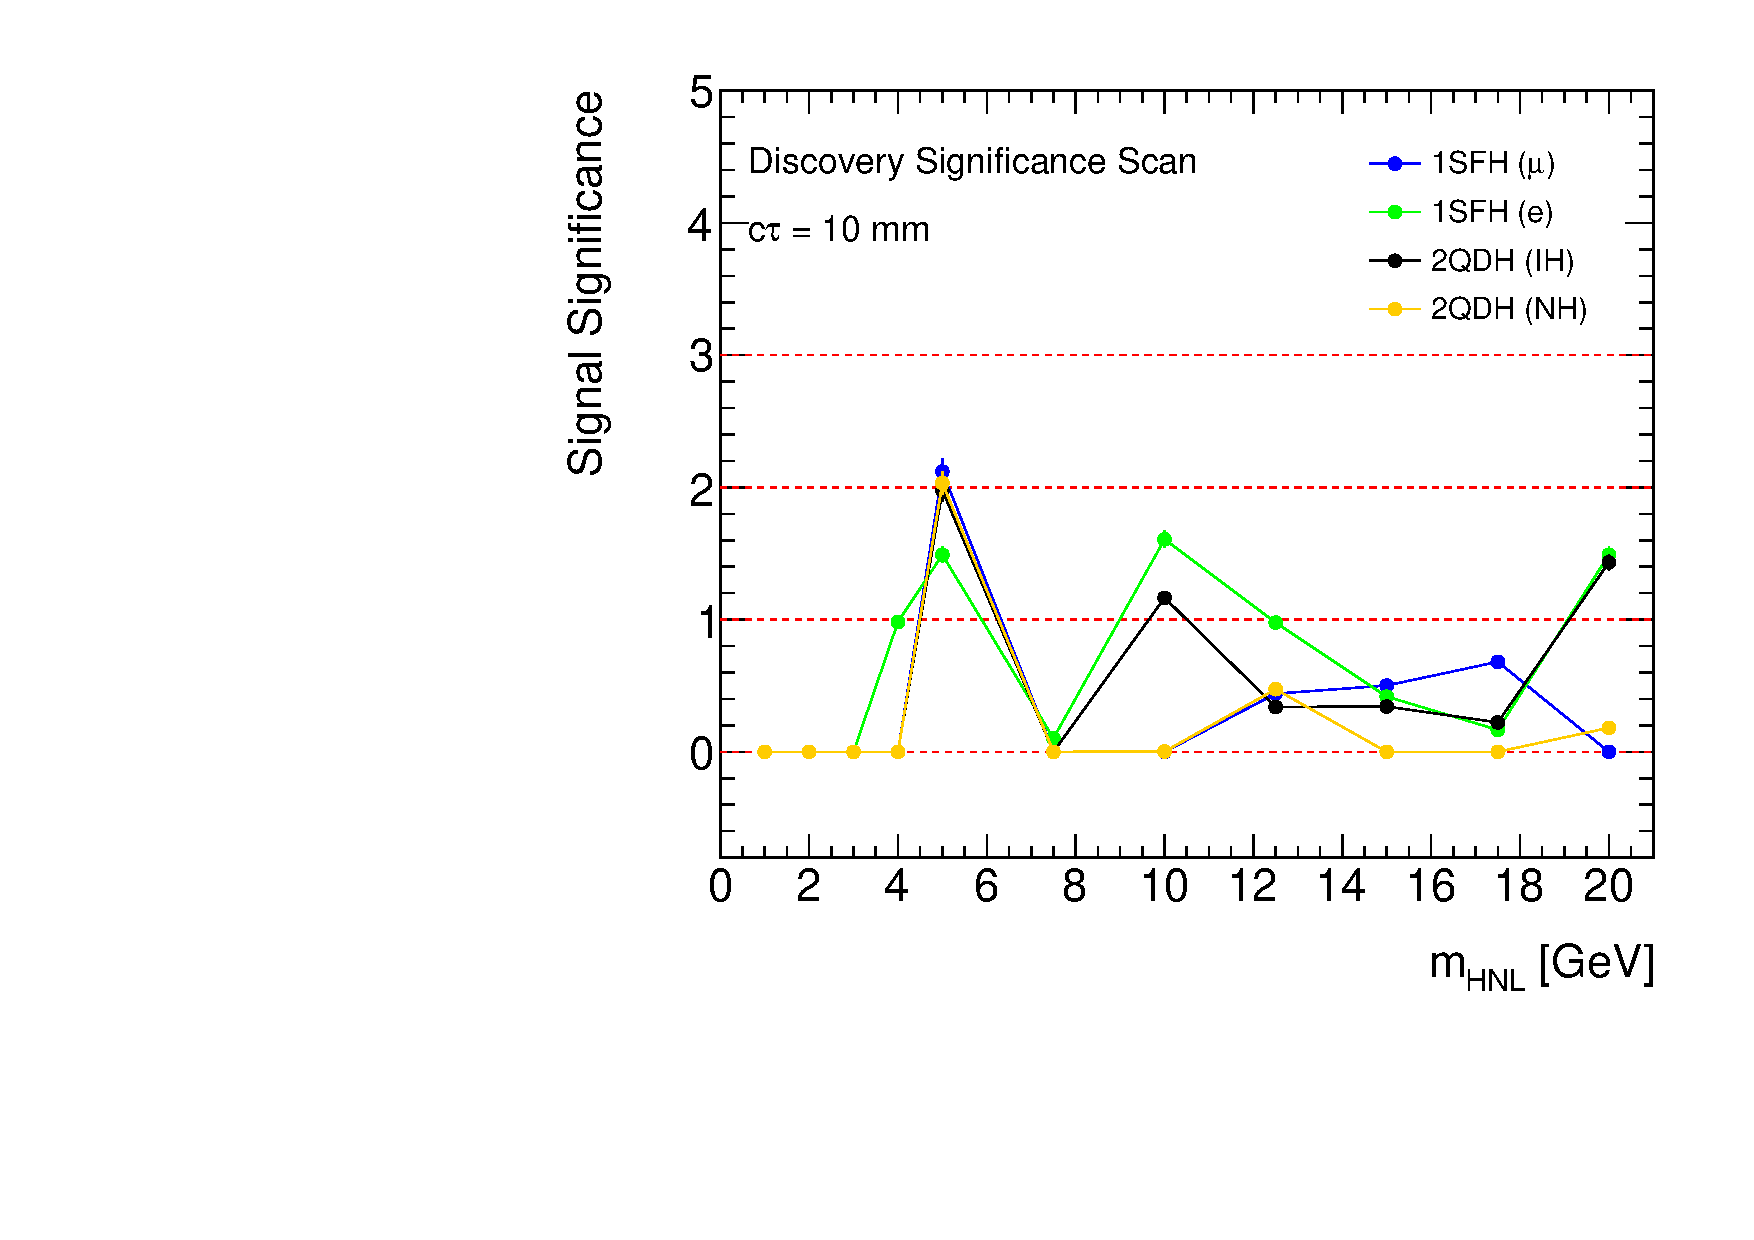
\includegraphics[width=0.5\textwidth]{figures/results/signi_fixed_10.pdf}}
    \subfloat[\ctau = 100 mm]{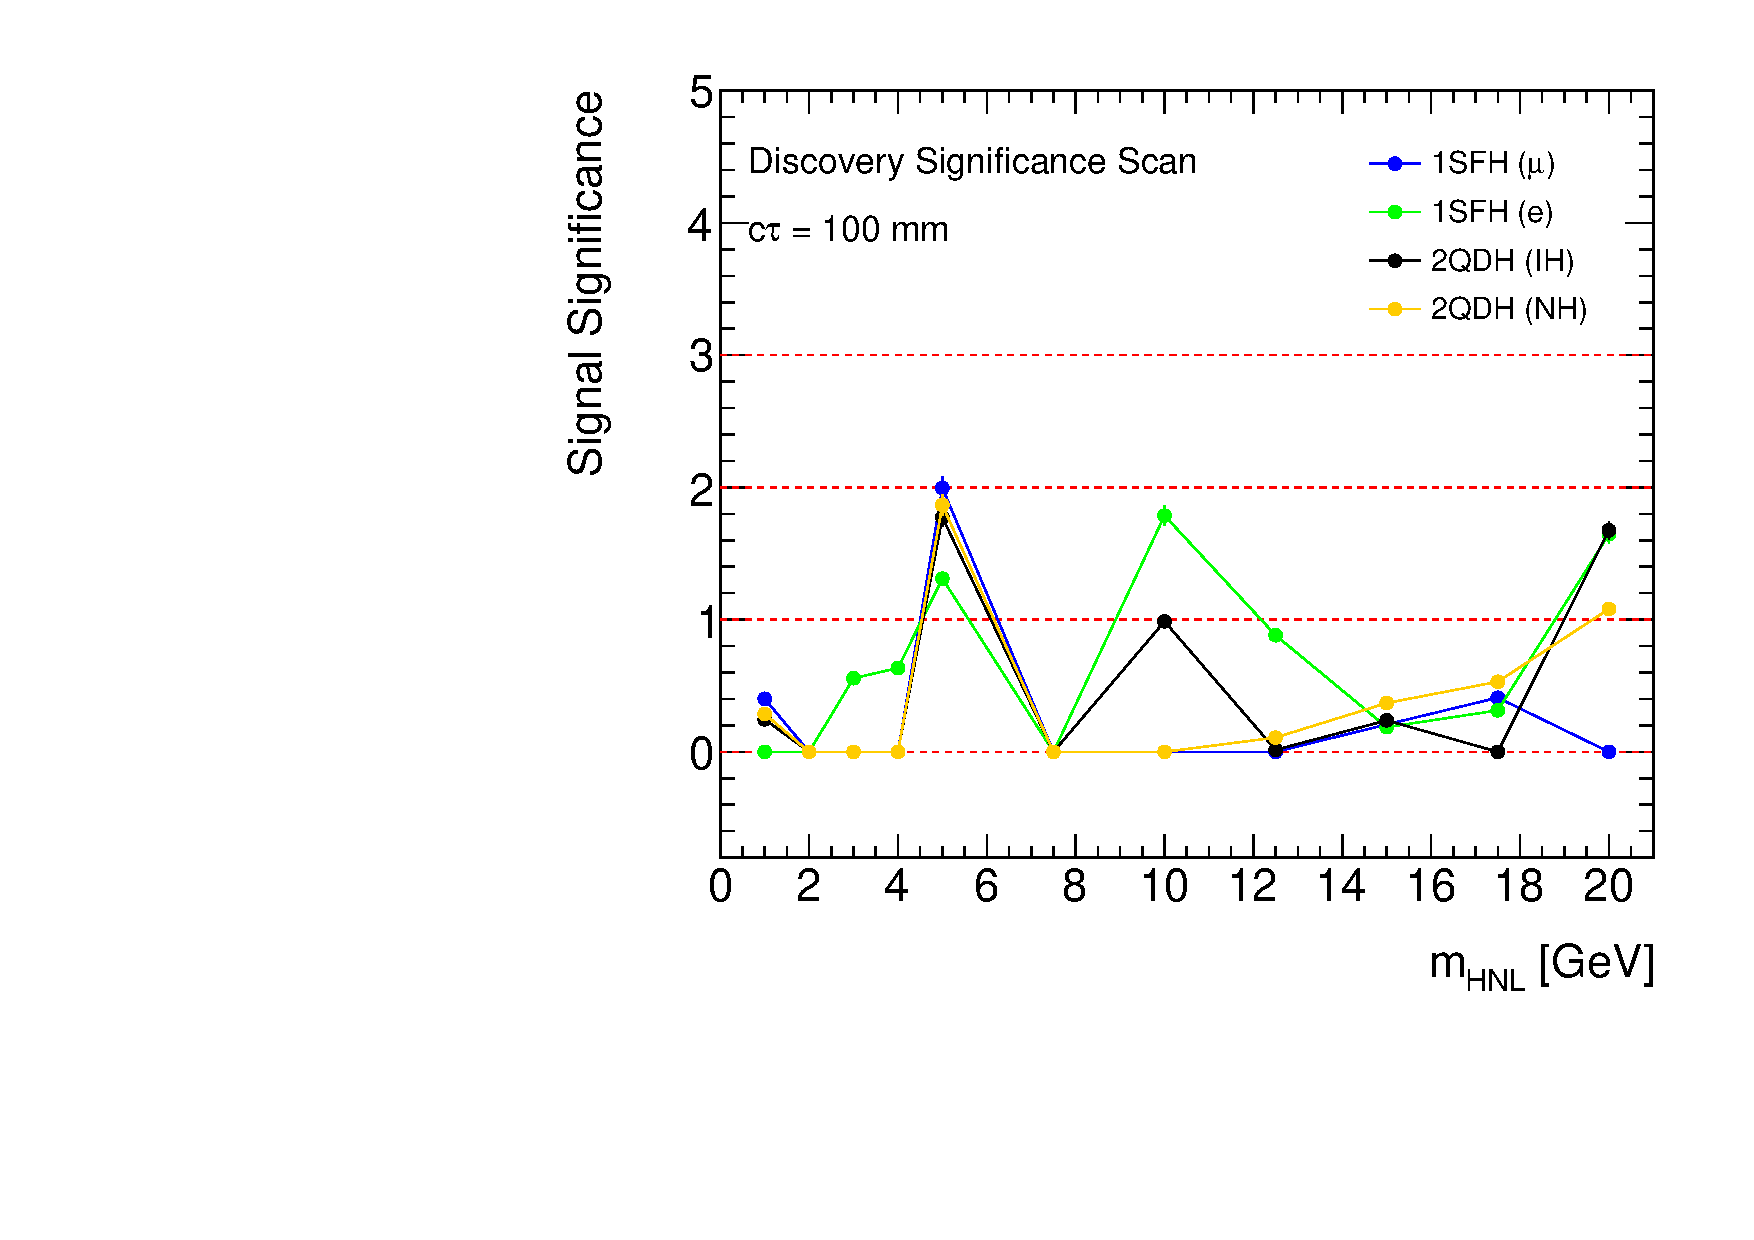
\includegraphics[width=0.5\textwidth]{figures/results/signi_fixed_100.pdf}}
    \caption{Discovery significance as a function of mass for two representative HNL lifetimes for the four models considered. Negative significance values are shifted to zero.}
    \label{fig:disco_signi}
\end{figure}

The discovery significances across the mass spectrum are seen to be compatible for the 10 mm and 100 mm samples accounting for shape differences in the signal template from acceptance and efficiency effects of analysis cuts. There are three main features of the observed data events and the predicted background yields (see~\cref{fig:pre_fit_SR}) in the signal region which affect and explain the observed discovery significance:
\begin{enumerate}
    \item Under-fluctiation of background prediction: No data is observed in the SR of all channels up to $\mhnl=2.5$~GeV and in $\mhnl=5-8$~GeV in the \uue SR. The non-negligible background predictions in these regions cause a $\hat{\mu}<0$ to be possible, and hence negative significances are observed in models that leave signatures in these mass ranges in the relevant channels.
    \item Outliers described in~\cref{tab:outlying_events_kinem}: The $\mhnl=19.1$~GeV event in the \euu channel creates a positive significance at the level of 1.5 standard deviations in the 1SFH($e$) and 2QDH(IH) model, since the 1SFH($\mu$) model does not have signal events in the \euu channel and the contribution from the 2QDH(NH) is also low, since it has a much higher coupling to muons than electrons. The $\mhnl=16$~GeV event does not cause a significant excess, since the simulated points are at 15 and 17.5 GeV, which only have their mass tails at the outlying point. The last outlier event at 9.6 GeV in the \eeu channel also creates a positive significance of about 1.5 standard deviations in the 1SFH($e$) and 2QDH(IH) models, while the other two models that are largely coupled to muons are not sensitive to this event.
    \item Excess around $\mhnl=5$~GeV: In all channels at varying degrees, a slight pre-fit underestimation of data by the background estimate around $\mhnl=4-6$~GeV is observed. This excess of data causes a signal significance observation of 2 standard deviations for all models except 1SFH($e$), which is at the level of 1.5 standard deviations. A possible reason for such an effect is the shape building process of the HF background in the SR, where all channels are combined to build the template shape, with the underlying educated assumption that the HF background has a similar signature irrespective of the lepton flavor.
\end{enumerate}

The discovery significance study shows \textbf{no deviation beyond statistical fluctuations} in this measurement, even though there are isolated excesses which could have been significant. This shows the strength of the analysis method where the signal is extracted using multiple regions at once using the \mhnl shape, where both of these techniques (simultaneous fit and the \mhnl shape) reduce the influence of such fluctuations on the overall measurement.

\begin{table}[!htbp]
    \centering
    \begin{tabular}{c|ccc|ccc}
    \hline \hline
    \multirow{2}{*}{Channel} & \multicolumn{3}{c|}{Signal Region} & \multicolumn{3}{c}{Control Region} \\
    \cline{2-7}
    & Hadrons & Crossings & Obs. & Hadrons & Crossings & Obs. \\
    \hline
    \uuu & $23.1\pm2.6$ & $0.023\pm0.012$ & 23 & $254.4\pm13.4$ & $0.16\pm0.08$ & 261 \\
    \uue & $9.2\pm0.8$ & $0.016\pm0.008$ & 5 & $135.3\pm7.9$ & $0.096\pm0.052$ & 134 \\
    \uee & - & - & - & $23.7\pm2.5$ & $0.015\pm0.008$ & 27 \\
    \euu & $25.9\pm1.7$ & $0.0014\pm0.0007$ & 26 & $248.8\pm12.1$ & $0.051\pm0.028$ & 252 \\
    \eeu & $9.6\pm0.9$ & $0.027\pm0.015$ & 13 & $153.3\pm8.7$ & $0.057\pm0.030$ & 149 \\
    \eee & - & - & - & $22.4\pm2.8$ & $0.094\pm0.050$ & 24 \\
    \xee & $0.22\pm0.14$ & $0.043\pm0.023$ & 1 & - & - & - \\
    \hline \hline 
    \end{tabular} 
    \caption{Post-fit yields of heavy flavor hadron decay background (Hadrons), random crossing background (Crossings), and data (Obs.) in the signal and control regions using the $\mhnl=5$~GeV, $\ctau=10$~mm 2QDH(IH) model as a benchmark.} 
    \label{tab:post_fit_yields}
\end{table} 

~\Cref{tab:post_fit_yields} shows the post-fit yields for the observed data and background processes obtained using the $\mhnl=5$~GeV, $\ctau=10$~mm samples in the 2QDH(IH) model as a benchmark. The simultaneous fit gives a signal strength of $\hat{\mu}=0.041\pm0.024$ and a HF background normalization of $\hat{\mu_b}=1.16\pm0.11$. This model is easily excluded, as is shown in the next section.

~\Cref{tab:uncertainty} shows the percent impact of the sources of uncertainties considered in this analysis obtained using the 2QDH(IH) model for HNL masses and lifetimes at the edge of the exclusion contour (see~\cref{sec:limits}). As expected, the random crossing estimate becomes relevant only at larger \mhnl, since the HF background dominates at relatively lower masses. At very low masses where there is no contribution from the HF background, the signal modeling and lepton measurement systematics dominate. Overall, however, the impact of systematic uncertainties is significantly smaller than the statistical uncertainty.

\begin{table}[!htbp]
    \centering
    \resizebox{\columnwidth}{!}{
    \begin{tabular}{ccccc}
        \hline\hline
        \multirow{2}{*}{Uncertainty Source} & \multicolumn{4}{c}{Impact (\%) on $\hat{\mu}$ using 2QDH(IH) (\mhnl, \ctau)} \\
        & 1 GeV, 1000 mm & 3 GeV, 1 mm & 5 GeV, 10 mm & 12.5 GeV, 10 mm \\
        \hline
        Leptons & 2.7 & 2.0 & 4.5 & 2.7 \\
        Flavor Tagging & $<0.1$ & 1.3 & 1.5 & 0.4 \\
        Pileup & 1.1 & 1.1 & 3.3 & $<0.1$ \\
        Luminosity & 0.3 & 0.3 & 0.6 & 0.3 \\
        \hline
        Signal Modeling & 1.7 & 1.8 & 3.4 & 1.8 \\
        HF Bkg. Modeling & 0.2 & 9.1 & 9.6 & 1.1 \\
        RC Bkg. Modeling & $<0.1$ & $<0.1$ & $<0.1$ & 24.2 \\
        \hline
        HF Bkg. Template & 0.4 & 2.9 & 3.9 & 1.1 \\
        Signal MC Stats. & 12.2 & 3.2 & 3.4 & 3.1 \\
        HF Normalization & 1.2 & 2.4 & 1.3 & 1.3 \\
        \hline
        Total Syst. & 12.7 & 11.0 & 12.6 & 4.8 \\
        Data Stats. & 94.7 & 112.5 & 33.0 & 175.5 \\
        \hline
        Total & 95.5 & 113.0 & 35.3 & 175.6 \\
        \hline \hline
    \end{tabular}
    }
    \caption{Percentage impact of uncertainties on the measured signal strength $\hat{\mu}$ for the 2QDH(IH) HNL model for representative mass and proper lifetimes at the edges and in the bulk of the sensitivity.}
    \label{tab:uncertainty}
\end{table}

\section{Exclusion Limits}\label{sec:limits}

Since no deviations beyond statistical fluctuations are found, 95\% CL upper limits of the signal strength are obtained for the four benchmark models, and the exclusion contours are shown in~\cref{fig:limits}. The limits are obtained using the ``Asymptotic" method~\cite{Cowan:2010js} which performs an analytical calculation using a $\chi^2$ approximation of $q_{\mu}$. A comparison of using the Aymptotic method against pseudo-experiments is shown in~\cref{chap:asymp_vs_toys} of the appendix. The figures show the observed and expected exclusion contours as a function of the HNL mass and the square of mixing to SM neutrinos ($|U|^2$), and the same is compared to the expected exclusion from the 2022 analysis. All the mass and couplings within the contour are excluded from possible HNL models.

\begin{figure}[!htbp]
    \centering
    \subfloat[1SFH($e$)]{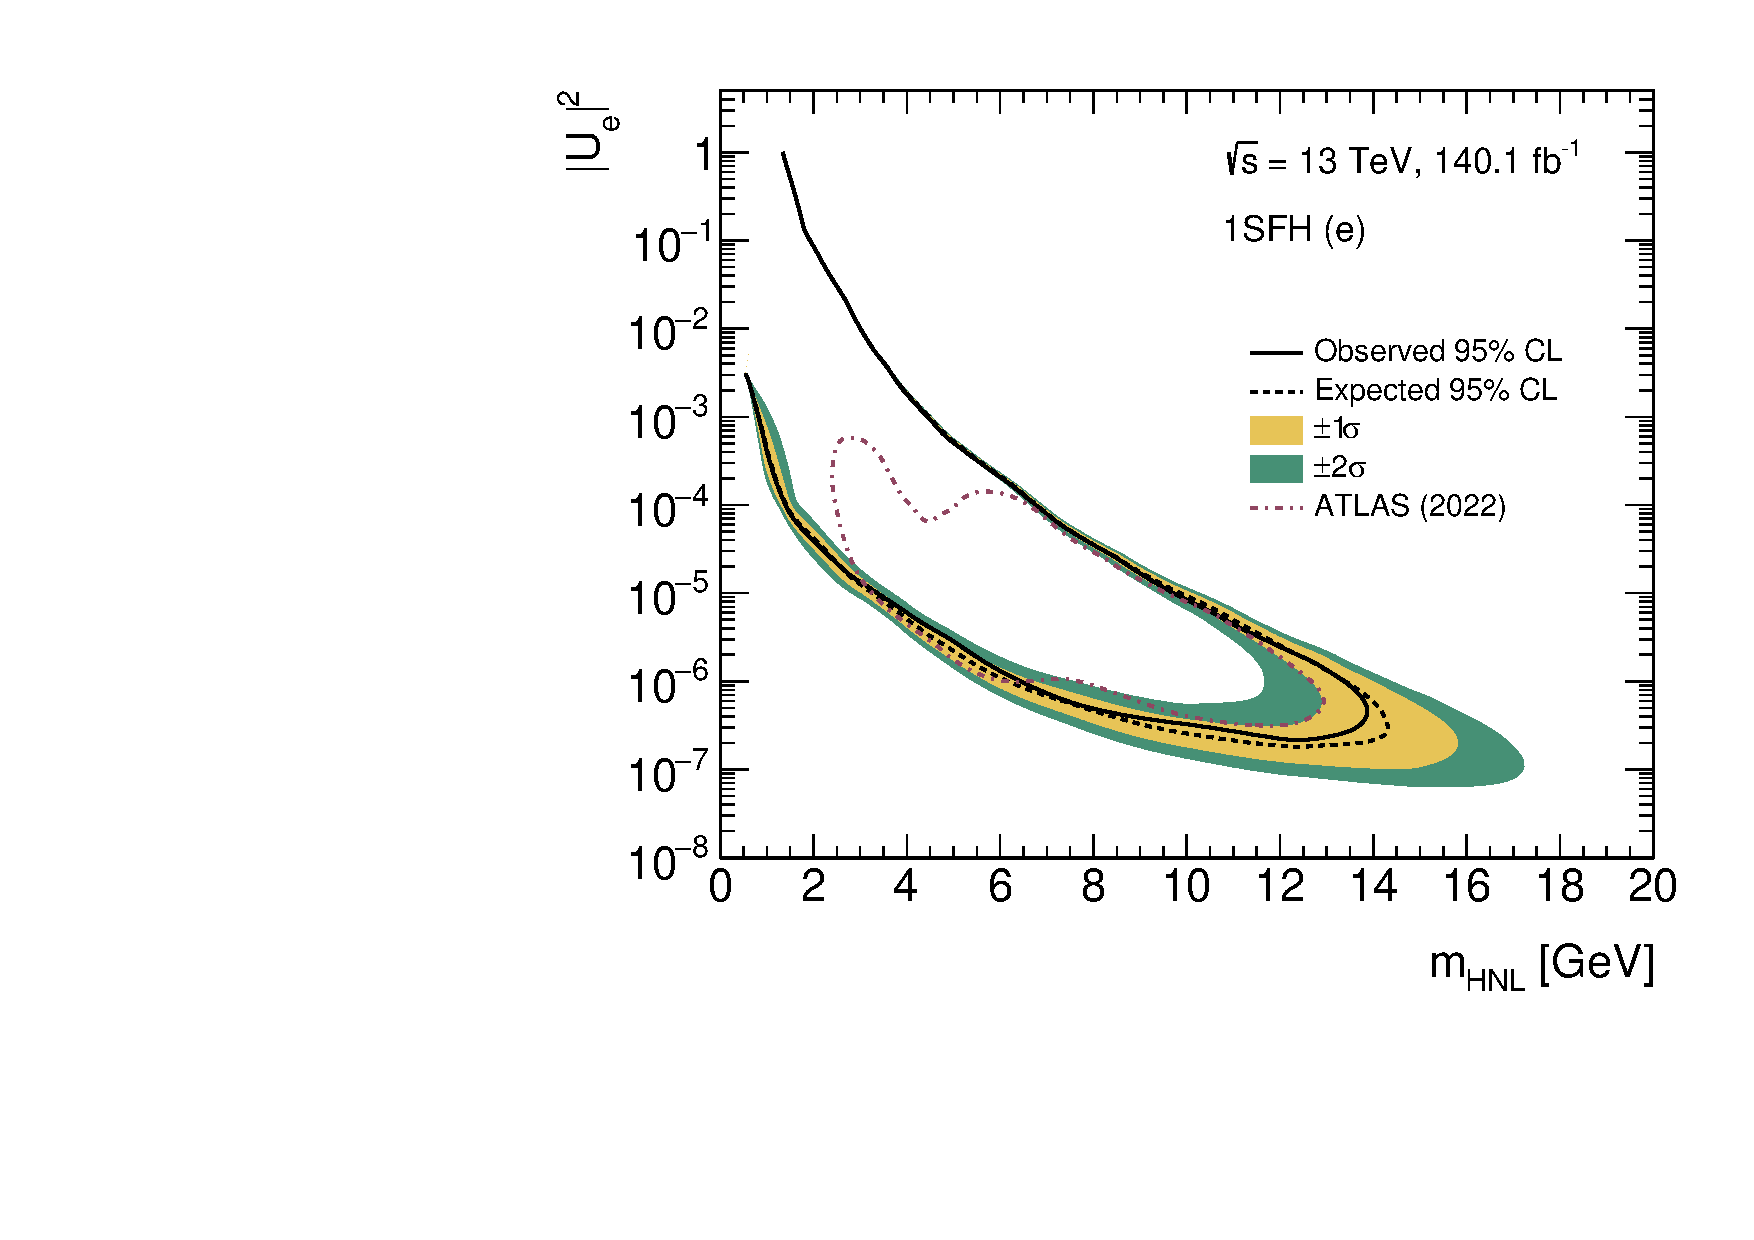
\includegraphics[width=.5\textwidth]{figures/results/limits_M_LNCpLNV_SF_el.pdf}}
    \subfloat[1SFH($\mu$)]{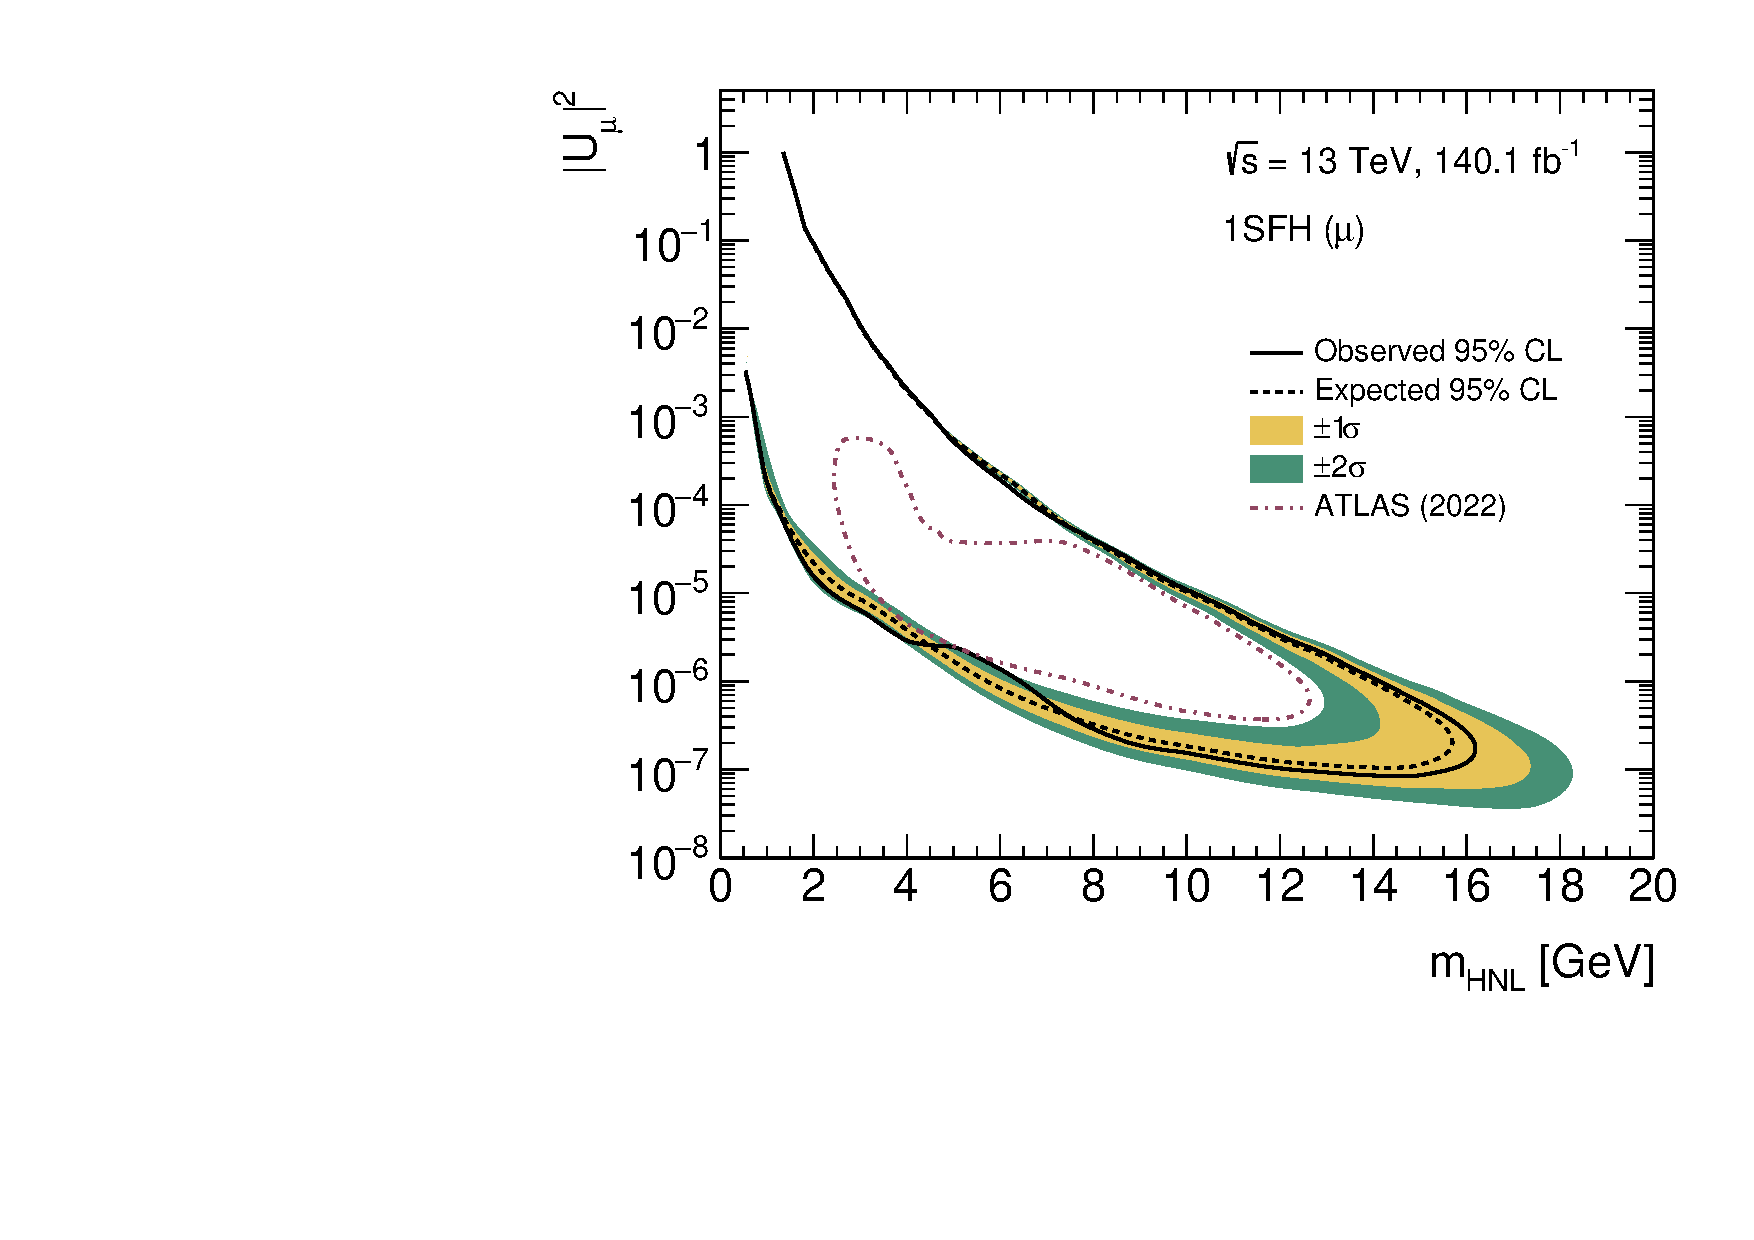
\includegraphics[width=.5\textwidth]{figures/results/limits_M_LNCpLNV_SF_mu.pdf}}\\
    \subfloat[2QDH(IH)]{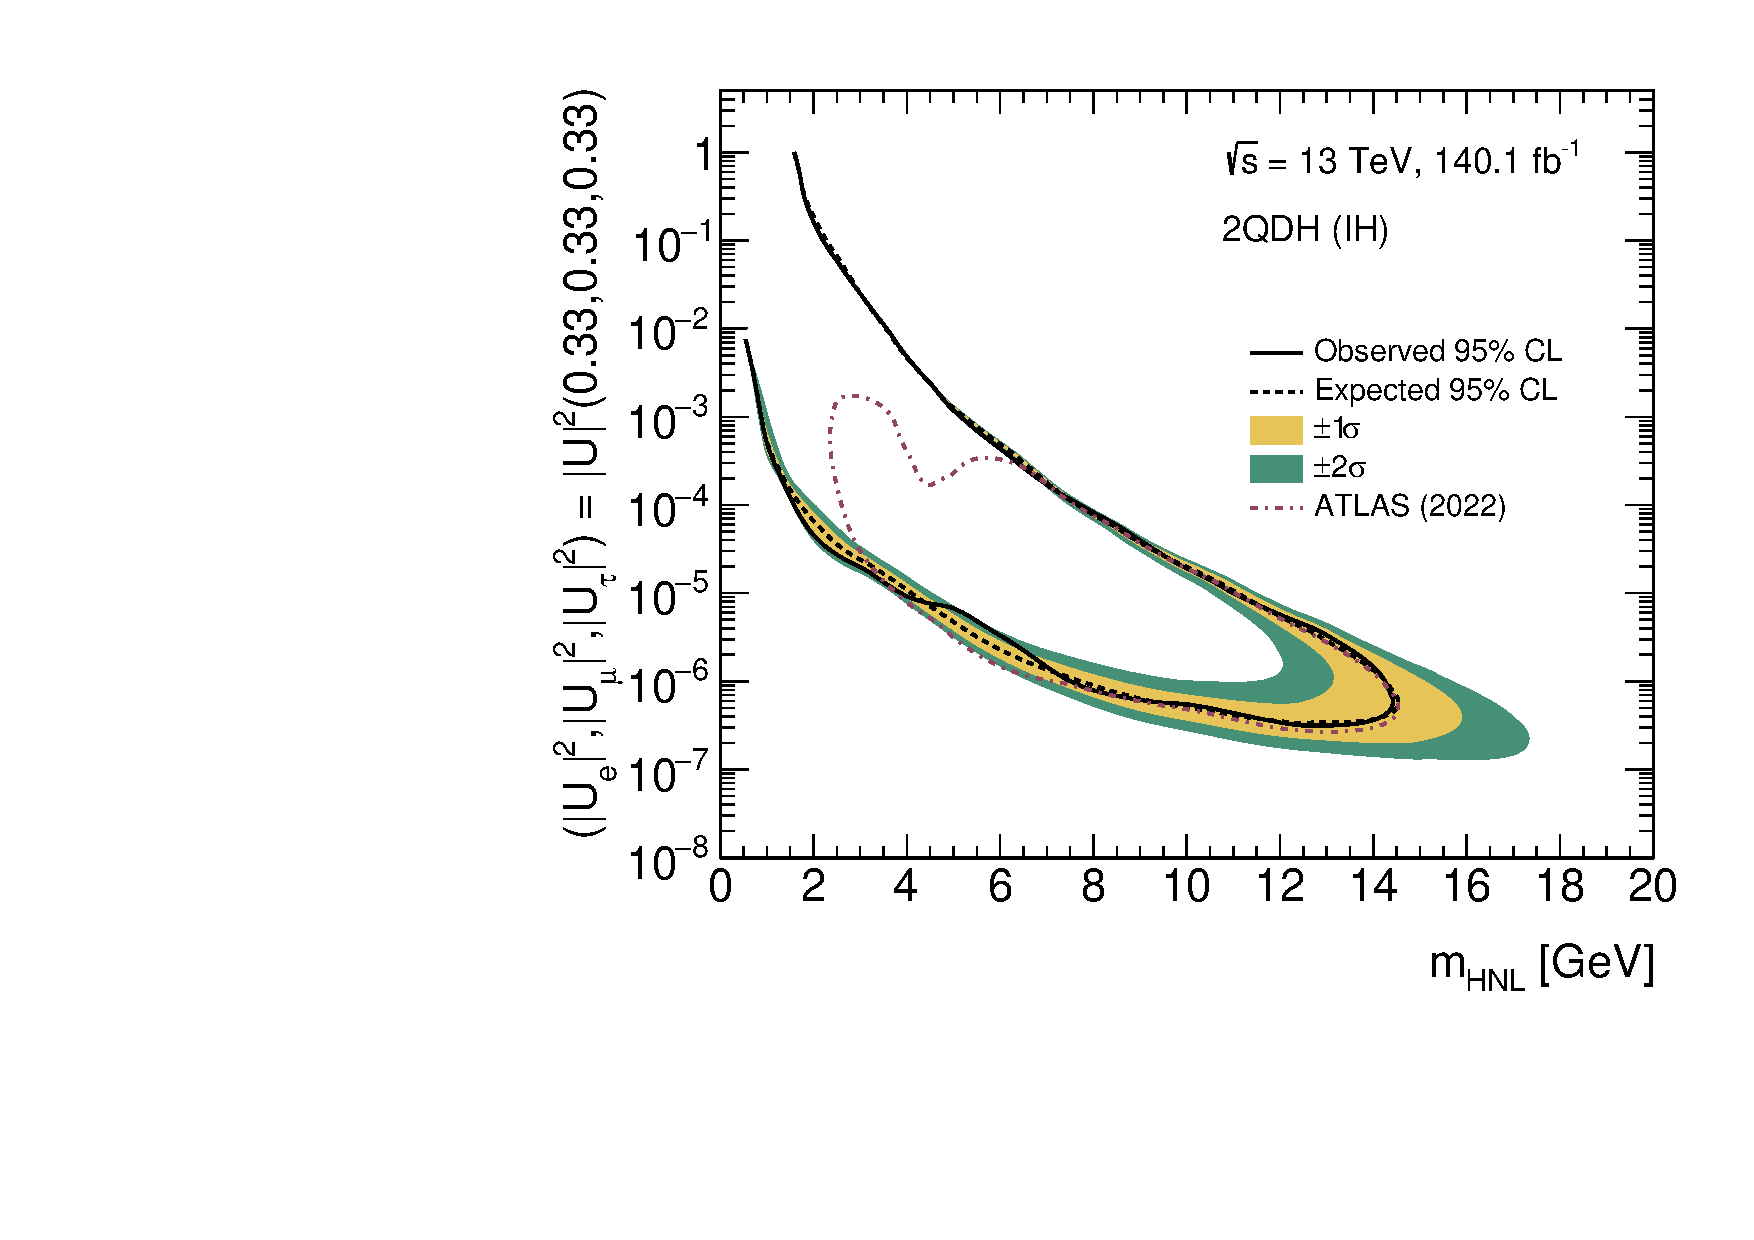
\includegraphics[width=.5\textwidth]{figures/results/limits_MQD_LNCpLNV_IH.pdf}}
    \subfloat[2QDH(NH)]{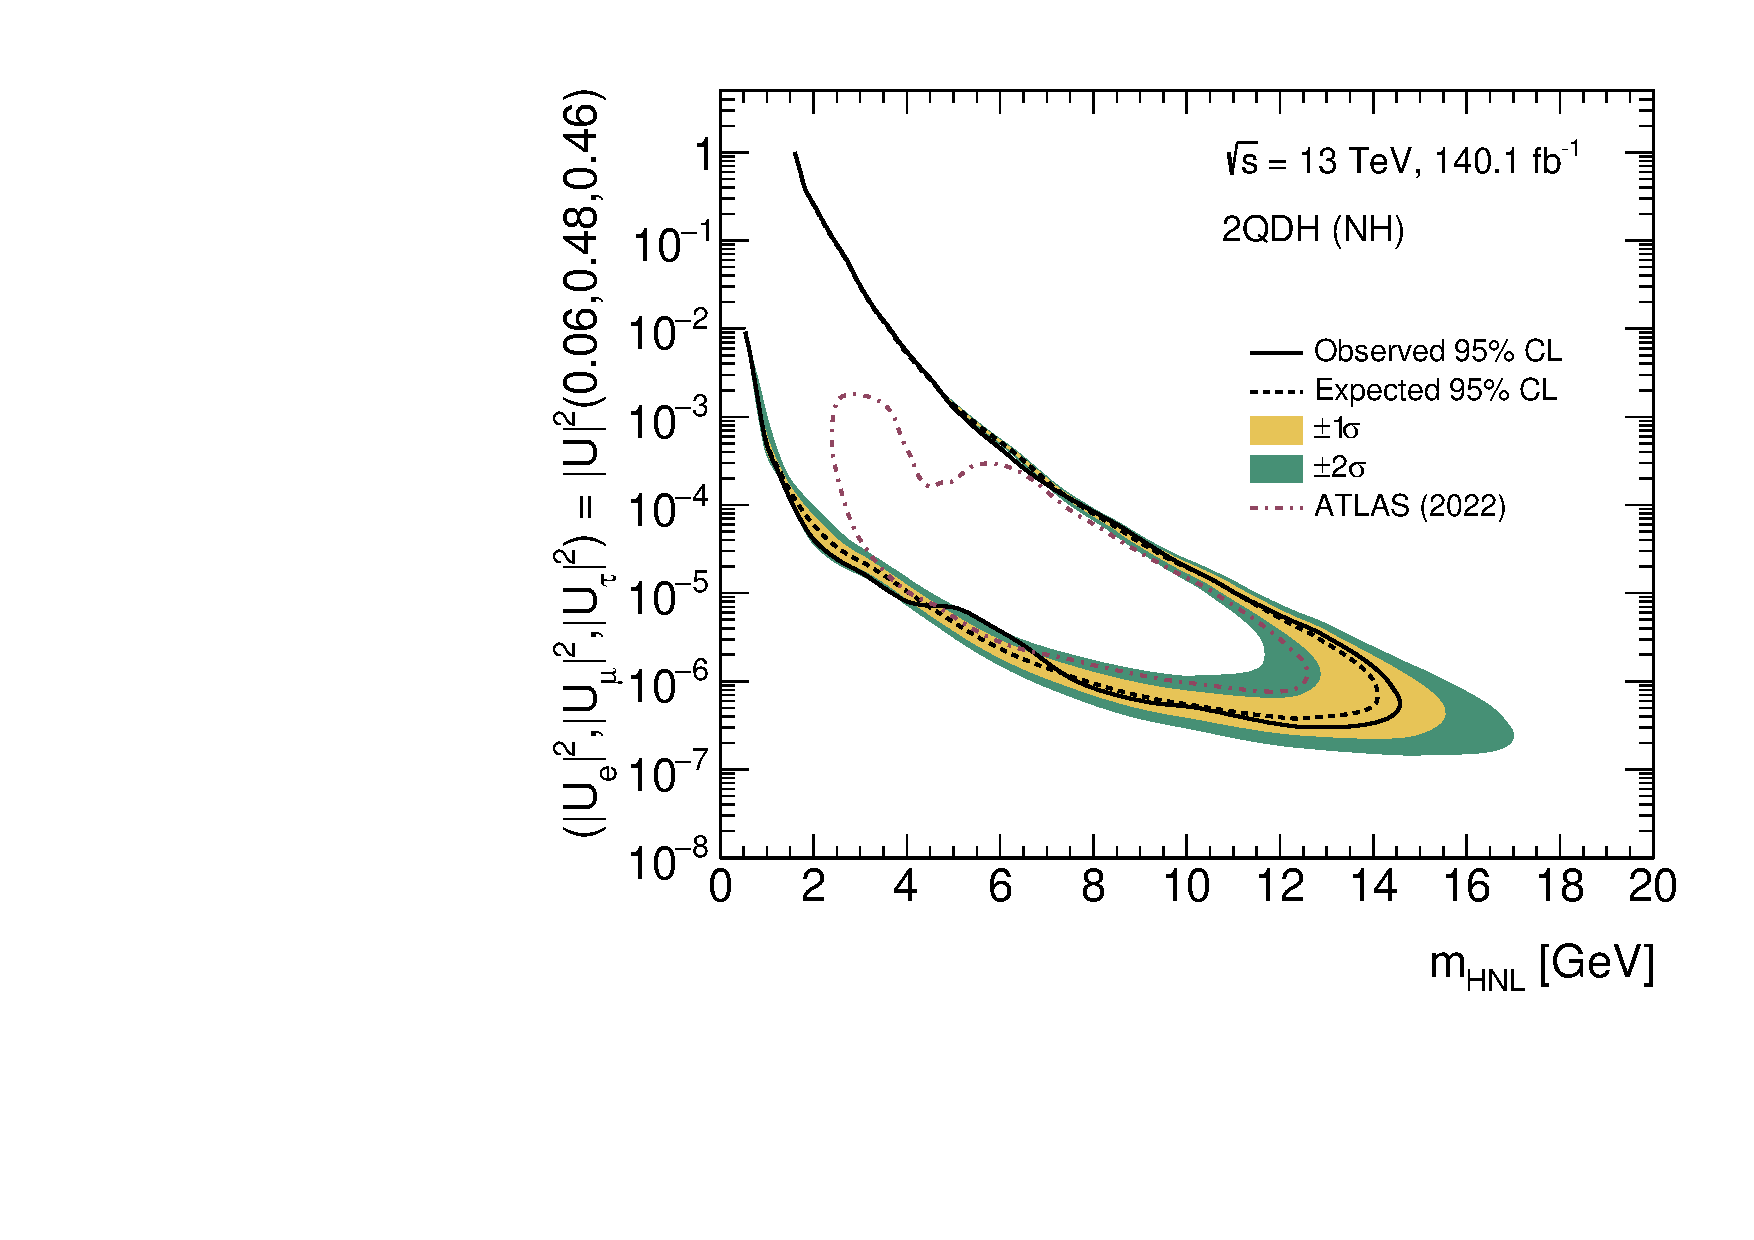
\includegraphics[width=.5\textwidth]{figures/results/limits_MQD_LNCpLNV_NH.pdf}}
    \caption{The observed (solid line) and expected (dashed line) 95\% exclusion contours for the four benchmark models as a function of the HNL mass and $|U|^2$. The green and yellow bands shows the range of limits within 1 and 2 standard deviations, respectively. The violet dashed line shows the expected exclusion contour of the 2022 analysis.}
    \label{fig:limits}
\end{figure}

The shape the contour is well explained by the relationship between $|U|^2$, the HNL proper lifetime, and the HNL mass, $\tau_\mathrm{HNL} \propto \frac{1}{\mhnl^5 |U|^2}$. The analysis shows sensitivity to models with $\ctau=1-1000$~mm, corresponding to mixing angles as low as $10^{-6}$ up to $\mhnl=5$~GeV. HNLs with larger lifetimes do not have enough decays in the ID volume for the analysis to be sensitive to them. HNLs with shorter lifetime fail the $\rdv>4$~mm requirement since they are not displaced enough to be captured by the secondary vertex selection. As the mass increases, the HNL production cross-section reduces, decreasing the overall sensitivity to these HNLs. The 1SFH($\mu$) contour shows an impressive level of exclusion where a 16 GeV HNL is excluded for mixing angles as low as $10^{-7}$, a region untouched by other measurements. The contour is open in the low mass end since there is no estimate of the level of exclusion for $\mhnl<1$~GeV. To provide measurable (but not unphysically) large couplings, HNLs with smaller ($<1$~GeV) masses require very large proper lifetimes to which the analysis has no acceptance. 
%Furthermore, the resolution of mass measurement using a DV reconstruction is not small enough to precisely measure such small masses. 
The $\mhnl=1$~GeV, $\ctau=1000$~mm HNLs are excluded for all models, a lifetime not excluded for any mass in the 2022 analysis. The expected and observed exclusions are compatible with each other. However, the observed exclusion has a slight dip in the $\mhnl=6-8$~GeV region. This is precisely because of the excess/peak shift effect around 5 GeV that was described in~\cref{sec:event_excess}, where a larger amount of data is observed than the background prediction. Nevertheless, no excess beyond two-standard deviation level is measured, as was also verified by the discovery significance scans.

\begin{figure}[!htbp]
    \centering
    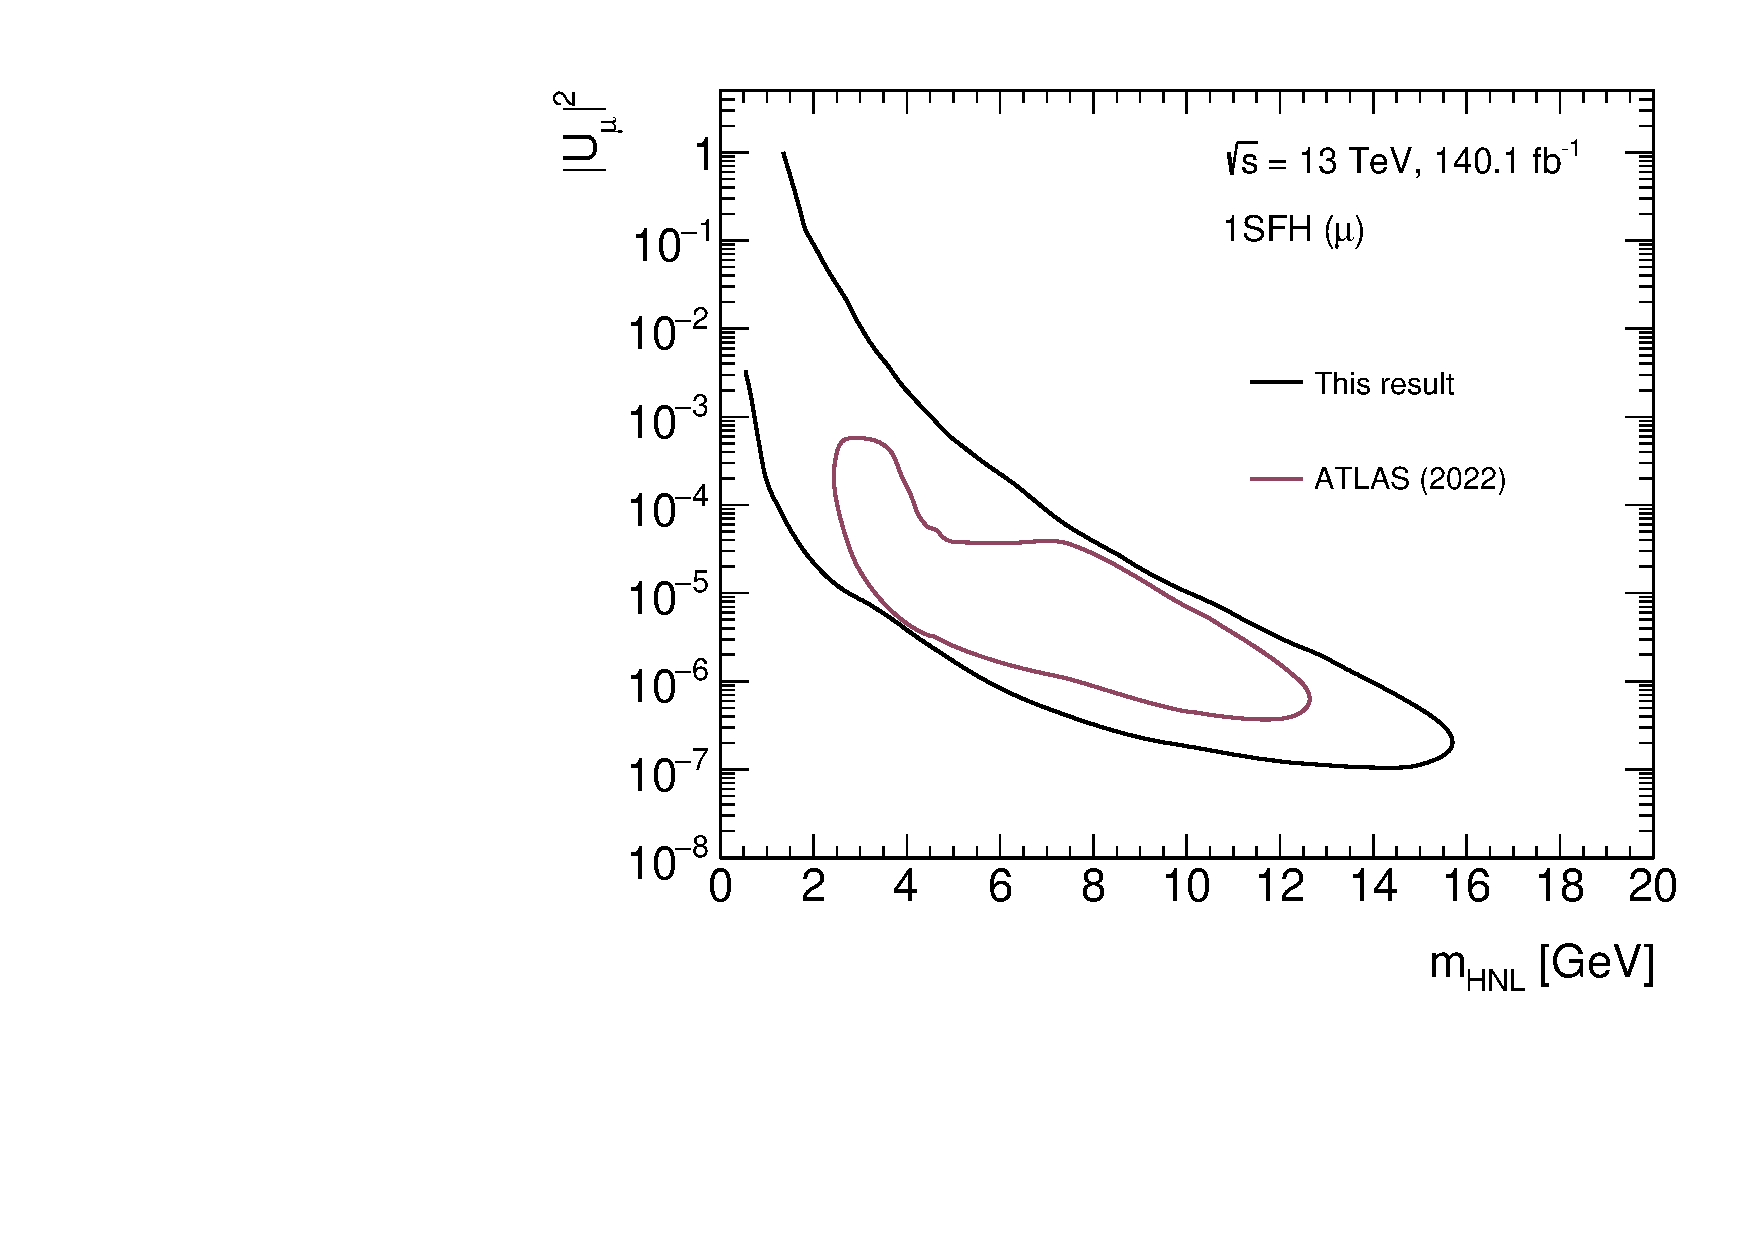
\includegraphics[width=.72\textwidth]{figures/results/limits_M_LNCpLNV_SF_mu_v_r21.pdf}\\
    \caption{The expected 95\% exclusion contours for the 1SFH($\mu$) HNL model as a function of the HNL mass and $|U|^2$ for this result (black) and the 2022 analysis (violet).}
    \label{fig:mu_only_limit_vs_2022}
\end{figure}

~\Cref{fig:mu_only_limit_vs_2022} shows a simplified comparison of the expected exclusion from this result compared to the 2022 analysis. The improved reconstruction and analysis methods used in this analysis with respect to the 2022 analysis are apparent in the comparison. The first visible improvement is an extension of the sensitivity reach to the 1-3 GeV range. The 2022 analysis was forced to apply stringent cuts to reject the HF background which also added the ``kink" in their exclusion shape. The removal of this cut and the robust HF background estimation in my analysis allows for the significant improvement to sensitivity in the low mass region. For some models, the high mass exclusion extends up to 16 GeV, to be compared to 14 GeV in the 2022 analysis, thanks to the improvements to VSI (especially a bug fix which resulted in significantly lower random crossings), the improved LRT, and the use of \mhnl shape as a discriminant. The most significant difference between the two analyses is in the 1SFH($\mu$) model, where the exclusion contour is visibly expanded in all directions. The lowest mixing angle excluded by the 2022 analysis using the 1SFH($\mu$) model was at 12 GeV. This exclusion has been improved by an order of magnitude.